\documentclass[11pt]{article}
\usepackage[a4paper,margin=1in]{geometry}
\usepackage{amsmath,amssymb,amsthm}
\usepackage{tikz}
\usetikzlibrary{arrows.meta}
\usepackage{xcolor}
\usepackage{booktabs}
\usepackage[hidelinks]{hyperref}
\hypersetup{pdftitle={Wandering over the divisors of a power of ten},pdfauthor={Vamshi Jandhyala}}
\setlength{\parskip}{0.4em}
\setlength{\parindent}{0pt}

\newtheorem{theorem}{Theorem}
\newtheorem{lemma}[theorem]{Lemma}
\newtheorem{corollary}[theorem]{Corollary}
\newtheorem{conjecture}[theorem]{Conjecture}
\theoremstyle{remark}
\newtheorem*{remark}{Remark}

\definecolor{inkblue}{RGB}{40,76,105}
\definecolor{rust}{RGB}{153,70,45}

\newcommand{\E}{\mathsf{E}}
\newcommand{\N}{\mathsf{N}}
\newcommand{\D}{\mathsf{D}}

\title{Wandering over the divisors of a power of ten}
\author{Vamshi Jandhyala}
\date{}

\begin{document}
\maketitle
\vspace{-2em}

\begin{abstract}
A referee names a divisor of $10^n$. Two players then take turns multiplying the last number
named by $2$ or by $5$, or dividing it by $10$, always naming a divisor of $10^n$ that nobody has
named before; the player who cannot move loses. The game comes from the 2020 All-Ukrainian
Tournament of Young Mathematicians, which asks for the probability that the first player wins
when the referee's choice is random. It is equivalent to moving a piece on an $(n+1)\times(n+1)$
board with the steps $(1,0)$, $(0,1)$ and $(-1,-1)$. This note collects what can be proved and
what can be computed. For $n=6$ the first player wins with probability $29/49$, and the
pattern suggested by small boards, that the second player wins exactly from the squares with
both coordinates even when $n$ is even, fails from $n=6$ on. On every board the second player
wins against the opening $(1,0)$ or $(0,1)$ from a diagonal square, and against the opening
$(0,1)$ from a square of the bottom row; the strategies climb diagonals and sweep the edges of
the board. The general classification remains open, and the note records the data and the
approaches that fail.
\end{abstract}

\section{The game}

In 2020 a tournament for school students set a game on the divisors of $10^n$ and asked how
likely the first player is to win. The small cases suggest a tidy answer. That answer is wrong
from $10^6$ on, and the right one is not known. This note proves what it can about who wins,
and records what the computer says.

Write a divisor of $10^n$ as $2^x5^y$ with $0\le x,y\le n$ and place it on the square $(x,y)$
of the board $\{0,\dots,n\}^2$. Multiplying by $2$ moves the piece one square east, multiplying
by $5$ moves it one square north, and dividing by $10$ moves it one square diagonally south-west
(Figure~\ref{fig:moves}). Write $\E=(1,0)$, $\N=(0,1)$ and $\D=(-1,-1)$. The starting square
counts as named, a square may not be entered twice, and the player to move with no legal move
loses. Call the player who moves first Alice and the other Bob. A starting square is
\emph{losing} (L) when Bob has a winning strategy from it and \emph{winning} (W) otherwise.

\begin{figure}[ht]
\centering
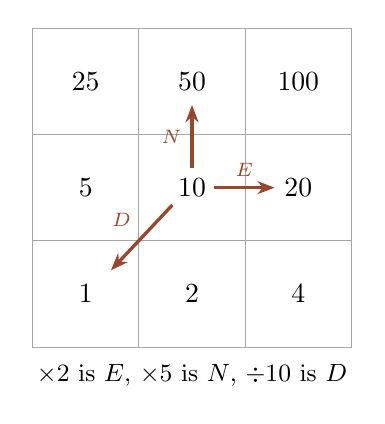
\begin{tikzpicture}[>={Stealth[length=2.2mm]}]
\draw[gray!70] (0.0,0.0) rectangle ++(1.35,1.35);
\node at (0.675,0.675) {$1$};
\draw[gray!70] (0.0,1.35) rectangle ++(1.35,1.35);
\node at (0.675,2.0250000000000004) {$5$};
\draw[gray!70] (0.0,2.7) rectangle ++(1.35,1.35);
\node at (0.675,3.375) {$25$};
\draw[gray!70] (1.35,0.0) rectangle ++(1.35,1.35);
\node at (2.0250000000000004,0.675) {$2$};
\draw[gray!70] (1.35,1.35) rectangle ++(1.35,1.35);
\node at (2.0250000000000004,2.0250000000000004) {$10$};
\draw[gray!70] (1.35,2.7) rectangle ++(1.35,1.35);
\node at (2.0250000000000004,3.375) {$50$};
\draw[gray!70] (2.7,0.0) rectangle ++(1.35,1.35);
\node at (3.375,0.675) {$4$};
\draw[gray!70] (2.7,1.35) rectangle ++(1.35,1.35);
\node at (3.375,2.0250000000000004) {$20$};
\draw[gray!70] (2.7,2.7) rectangle ++(1.35,1.35);
\node at (3.375,3.375) {$100$};
\draw[->, very thick, rust] (2.3050000000000006,2.0250000000000004) -- (3.0750000000000006,2.0250000000000004) node[midway, above] {\scriptsize $E$};
\draw[->, very thick, rust] (2.0250000000000004,2.2750000000000004) -- (2.0250000000000004,3.0750000000000006) node[midway, left] {\scriptsize $N$};
\draw[->, very thick, rust] (1.7750000000000004,1.8050000000000004) -- (0.9950000000000003,0.9750000000000003) node[midway, above left] {\scriptsize $D$};
\node[below] at (2.0250000000000004,-0.1) {\small $\times 2$ is $E$, $\times 5$ is $N$, $\div 10$ is $D$};
\end{tikzpicture}

\caption{The divisors of $10^2$ as a $3\times 3$ board, and the three moves from $10$.}
\label{fig:moves}
\end{figure}

Stop and try the $3\times3$ board before reading on. From the corner $1=(0,0)$ Alice must step
east or north, and Bob can always answer with the other step, landing on $(1,1)$ and then on
$(2,2)$; from $100=(2,2)$ the only move is back to $(1,1)$, which is taken. So $(0,0)$ is losing.
On this board the four corners are losing and the other five squares are winning.

The problem is question 20 of the 23rd All-Ukrainian Tournament of Young Mathematicians
(2020)~\cite{TYM}: the referee chooses the starting divisor at random, and the task is the
probability that Alice wins, (a) for $n=6$ and (b) for $n=2k$. Witold posted it on Mathematics
Stack Exchange~\cite{MSE}, and Vepir, who computed every board up to $11\times11$, asked about
the odd boards on MathOverflow~\cite{MO}. Their data suggested that for even $n$ the losing squares
are exactly those with both coordinates even, apart from a few sporadic squares, and Vepir
conjectured an exact pattern for odd $n$ with no sporadic squares at all. Vepir also proved by
hand that the corners are losing, and stated that $(2,0)$, $(0,2)$ and $(2,2)$ always are. No
solution of the tournament problem has been published.

Two facts are used throughout. Reflecting the board in the diagonal, $(x,y)\mapsto(y,x)$, swaps
$\E$ and $\N$ and fixes $\D$, so it maps the game to itself. And since $\E+\N+\D=0$, the three
squares $P$, $P+\E$, $P+\E+\N$ form a cycle of moves, as do $P$, $P+\N$, $P+\N+\E$: every
small triangle of the board, with the diagonal $(1,1)$ drawn in, is a directed $3$-cycle.

\section{Exact values on small boards}

An exhaustive search settles any single board. Two independent programs, one in C and one in
Python, solved every board up to $9\times 9$ and agree on every square; the C program also
solved the $10\times10$ board. Figure~\ref{fig:maps} shows three of the resulting maps.

\begin{figure}[ht]
\centering
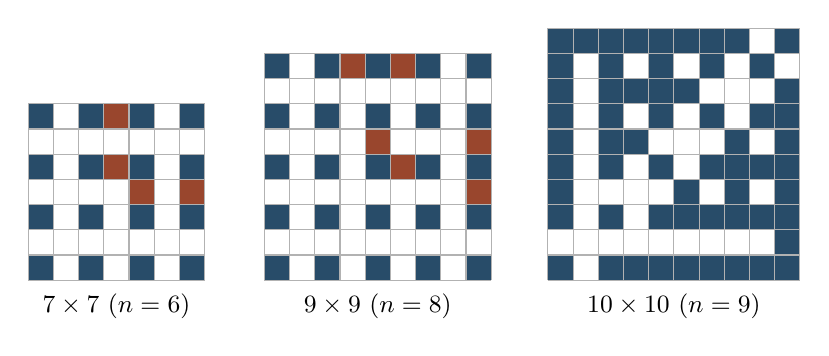
\begin{tikzpicture}
\begin{scope}[xshift=0.0cm]
\fill[inkblue] (0.000,0.000) rectangle ++(0.320,0.320);
\fill[inkblue] (0.000,0.640) rectangle ++(0.320,0.320);
\fill[inkblue] (0.000,1.280) rectangle ++(0.320,0.320);
\fill[inkblue] (0.000,1.920) rectangle ++(0.320,0.320);
\fill[inkblue] (0.640,0.000) rectangle ++(0.320,0.320);
\fill[inkblue] (0.640,0.640) rectangle ++(0.320,0.320);
\fill[inkblue] (0.640,1.280) rectangle ++(0.320,0.320);
\fill[inkblue] (0.640,1.920) rectangle ++(0.320,0.320);
\fill[rust] (0.960,1.280) rectangle ++(0.320,0.320);
\fill[rust] (0.960,1.920) rectangle ++(0.320,0.320);
\fill[inkblue] (1.280,0.000) rectangle ++(0.320,0.320);
\fill[inkblue] (1.280,0.640) rectangle ++(0.320,0.320);
\fill[rust] (1.280,0.960) rectangle ++(0.320,0.320);
\fill[inkblue] (1.280,1.280) rectangle ++(0.320,0.320);
\fill[inkblue] (1.280,1.920) rectangle ++(0.320,0.320);
\fill[inkblue] (1.920,0.000) rectangle ++(0.320,0.320);
\fill[inkblue] (1.920,0.640) rectangle ++(0.320,0.320);
\fill[rust] (1.920,0.960) rectangle ++(0.320,0.320);
\fill[inkblue] (1.920,1.280) rectangle ++(0.320,0.320);
\fill[inkblue] (1.920,1.920) rectangle ++(0.320,0.320);
\draw[gray!60, step=0.32] (0,0) grid (2.240,2.240);
\node[below] at (1.120,-0.05) {\small $7\times 7$ ($n=6$)};
\end{scope}
\begin{scope}[xshift=3.0cm]
\fill[inkblue] (0.000,0.000) rectangle ++(0.320,0.320);
\fill[inkblue] (0.000,0.640) rectangle ++(0.320,0.320);
\fill[inkblue] (0.000,1.280) rectangle ++(0.320,0.320);
\fill[inkblue] (0.000,1.920) rectangle ++(0.320,0.320);
\fill[inkblue] (0.000,2.560) rectangle ++(0.320,0.320);
\fill[inkblue] (0.640,0.000) rectangle ++(0.320,0.320);
\fill[inkblue] (0.640,0.640) rectangle ++(0.320,0.320);
\fill[inkblue] (0.640,1.280) rectangle ++(0.320,0.320);
\fill[inkblue] (0.640,1.920) rectangle ++(0.320,0.320);
\fill[inkblue] (0.640,2.560) rectangle ++(0.320,0.320);
\fill[rust] (0.960,2.560) rectangle ++(0.320,0.320);
\fill[inkblue] (1.280,0.000) rectangle ++(0.320,0.320);
\fill[inkblue] (1.280,0.640) rectangle ++(0.320,0.320);
\fill[inkblue] (1.280,1.280) rectangle ++(0.320,0.320);
\fill[rust] (1.280,1.600) rectangle ++(0.320,0.320);
\fill[inkblue] (1.280,1.920) rectangle ++(0.320,0.320);
\fill[inkblue] (1.280,2.560) rectangle ++(0.320,0.320);
\fill[rust] (1.600,1.280) rectangle ++(0.320,0.320);
\fill[rust] (1.600,2.560) rectangle ++(0.320,0.320);
\fill[inkblue] (1.920,0.000) rectangle ++(0.320,0.320);
\fill[inkblue] (1.920,0.640) rectangle ++(0.320,0.320);
\fill[inkblue] (1.920,1.280) rectangle ++(0.320,0.320);
\fill[inkblue] (1.920,1.920) rectangle ++(0.320,0.320);
\fill[inkblue] (1.920,2.560) rectangle ++(0.320,0.320);
\fill[inkblue] (2.560,0.000) rectangle ++(0.320,0.320);
\fill[inkblue] (2.560,0.640) rectangle ++(0.320,0.320);
\fill[rust] (2.560,0.960) rectangle ++(0.320,0.320);
\fill[inkblue] (2.560,1.280) rectangle ++(0.320,0.320);
\fill[rust] (2.560,1.600) rectangle ++(0.320,0.320);
\fill[inkblue] (2.560,1.920) rectangle ++(0.320,0.320);
\fill[inkblue] (2.560,2.560) rectangle ++(0.320,0.320);
\draw[gray!60, step=0.32] (0,0) grid (2.880,2.880);
\node[below] at (1.440,-0.05) {\small $9\times 9$ ($n=8$)};
\end{scope}
\begin{scope}[xshift=6.6cm]
\fill[inkblue] (0.000,0.000) rectangle ++(0.320,0.320);
\fill[inkblue] (0.000,0.640) rectangle ++(0.320,0.320);
\fill[inkblue] (0.000,0.960) rectangle ++(0.320,0.320);
\fill[inkblue] (0.000,1.280) rectangle ++(0.320,0.320);
\fill[inkblue] (0.000,1.600) rectangle ++(0.320,0.320);
\fill[inkblue] (0.000,1.920) rectangle ++(0.320,0.320);
\fill[inkblue] (0.000,2.240) rectangle ++(0.320,0.320);
\fill[inkblue] (0.000,2.560) rectangle ++(0.320,0.320);
\fill[inkblue] (0.000,2.880) rectangle ++(0.320,0.320);
\fill[inkblue] (0.320,2.880) rectangle ++(0.320,0.320);
\fill[inkblue] (0.640,0.000) rectangle ++(0.320,0.320);
\fill[inkblue] (0.640,0.640) rectangle ++(0.320,0.320);
\fill[inkblue] (0.640,1.280) rectangle ++(0.320,0.320);
\fill[inkblue] (0.640,1.600) rectangle ++(0.320,0.320);
\fill[inkblue] (0.640,1.920) rectangle ++(0.320,0.320);
\fill[inkblue] (0.640,2.240) rectangle ++(0.320,0.320);
\fill[inkblue] (0.640,2.560) rectangle ++(0.320,0.320);
\fill[inkblue] (0.640,2.880) rectangle ++(0.320,0.320);
\fill[inkblue] (0.960,0.000) rectangle ++(0.320,0.320);
\fill[inkblue] (0.960,1.600) rectangle ++(0.320,0.320);
\fill[inkblue] (0.960,2.240) rectangle ++(0.320,0.320);
\fill[inkblue] (0.960,2.880) rectangle ++(0.320,0.320);
\fill[inkblue] (1.280,0.000) rectangle ++(0.320,0.320);
\fill[inkblue] (1.280,0.640) rectangle ++(0.320,0.320);
\fill[inkblue] (1.280,1.280) rectangle ++(0.320,0.320);
\fill[inkblue] (1.280,1.920) rectangle ++(0.320,0.320);
\fill[inkblue] (1.280,2.240) rectangle ++(0.320,0.320);
\fill[inkblue] (1.280,2.560) rectangle ++(0.320,0.320);
\fill[inkblue] (1.280,2.880) rectangle ++(0.320,0.320);
\fill[inkblue] (1.600,0.000) rectangle ++(0.320,0.320);
\fill[inkblue] (1.600,0.640) rectangle ++(0.320,0.320);
\fill[inkblue] (1.600,0.960) rectangle ++(0.320,0.320);
\fill[inkblue] (1.600,2.240) rectangle ++(0.320,0.320);
\fill[inkblue] (1.600,2.880) rectangle ++(0.320,0.320);
\fill[inkblue] (1.920,0.000) rectangle ++(0.320,0.320);
\fill[inkblue] (1.920,0.640) rectangle ++(0.320,0.320);
\fill[inkblue] (1.920,1.280) rectangle ++(0.320,0.320);
\fill[inkblue] (1.920,1.920) rectangle ++(0.320,0.320);
\fill[inkblue] (1.920,2.560) rectangle ++(0.320,0.320);
\fill[inkblue] (1.920,2.880) rectangle ++(0.320,0.320);
\fill[inkblue] (2.240,0.000) rectangle ++(0.320,0.320);
\fill[inkblue] (2.240,0.640) rectangle ++(0.320,0.320);
\fill[inkblue] (2.240,0.960) rectangle ++(0.320,0.320);
\fill[inkblue] (2.240,1.280) rectangle ++(0.320,0.320);
\fill[inkblue] (2.240,1.600) rectangle ++(0.320,0.320);
\fill[inkblue] (2.240,2.880) rectangle ++(0.320,0.320);
\fill[inkblue] (2.560,0.000) rectangle ++(0.320,0.320);
\fill[inkblue] (2.560,0.640) rectangle ++(0.320,0.320);
\fill[inkblue] (2.560,1.280) rectangle ++(0.320,0.320);
\fill[inkblue] (2.560,1.920) rectangle ++(0.320,0.320);
\fill[inkblue] (2.560,2.560) rectangle ++(0.320,0.320);
\fill[inkblue] (2.880,0.000) rectangle ++(0.320,0.320);
\fill[inkblue] (2.880,0.320) rectangle ++(0.320,0.320);
\fill[inkblue] (2.880,0.640) rectangle ++(0.320,0.320);
\fill[inkblue] (2.880,0.960) rectangle ++(0.320,0.320);
\fill[inkblue] (2.880,1.280) rectangle ++(0.320,0.320);
\fill[inkblue] (2.880,1.600) rectangle ++(0.320,0.320);
\fill[inkblue] (2.880,1.920) rectangle ++(0.320,0.320);
\fill[inkblue] (2.880,2.240) rectangle ++(0.320,0.320);
\fill[inkblue] (2.880,2.880) rectangle ++(0.320,0.320);
\draw[gray!60, step=0.32] (0,0) grid (3.200,3.200);
\node[below] at (1.600,-0.05) {\small $10\times 10$ ($n=9$)};
\end{scope}
\end{tikzpicture}

\caption{Losing squares (filled) with $(0,0)$ at the bottom left. On the odd boards, blue squares
have both coordinates even and rust squares are the exceptions. The $10\times 10$ board follows
Conjecture~\ref{conj:even} exactly.}
\label{fig:maps}
\end{figure}

\begin{theorem}\label{thm:counts}
For $n=2,4,6,8$ the number of losing squares is $4$, $9$, $20$ and $31$. In particular, if the
referee chooses a divisor of $10^6$ uniformly at random, Alice wins with probability $29/49$.
\end{theorem}

For $n=2k$ the squares with both coordinates even number $(k+1)^2$, which gives $4,9,16,25$.
The two counts part company at $n=6$, so the natural answer $1-(k+1)^2/(2k+1)^2$ to part (b) is
false. On the $7\times7$ board the extra losing squares are $(4,3)$, $(6,3)$ and their mirror
images; on the $9\times 9$ board they are $(5,4)$, $(8,3)$, $(8,5)$ and their mirror images.
No square with both coordinates even is winning on any board up to $9\times9$.

\section{Sweeping an edge}

Most of the strategies below end in the same way: the piece reaches the right-hand edge with the
column below it unused, and Bob walks it down.

\begin{lemma}\label{lem:sweep}
Suppose Alice is to move at $(n,y)$, that $y=n$ or $(n,y+1)$ has been named, and that for some
$m\le y$ the squares $(n,m),\dots,(n,y-1)$ are unnamed, where either $m=0$ or $(n-1,m-1)$ has been
named. Then Bob wins. The same holds with the coordinates exchanged, for the top row.
\end{lemma}

\begin{proof}
Induction on $y-m$. From $(n,y)$ the step $\E$ leaves the board and $\N$ leads to $(n,y+1)$,
which is named or off the board, so Alice's only possible move is $\D$ to $(n-1,y-1)$. When
$y=m$ that square is off the board or named, and Alice loses. When $y>m$, Bob answers $\E$ to
$(n,y-1)$, which is unnamed. Alice is now at $(n,y-1)$ with $(n,y)$ named and the same $m$, and
the induction hypothesis applies. The top row follows by reflection.
\end{proof}

With $y=n$ and $m=0$ this says: if Alice is to move at the corner $(n,n)$ and the right-hand
column below it is unused, Bob wins. Alice's forced move $\D$ is answered by $\E$, and so on down
the column; at $(n,0)$ she is stuck.

\section{Climbing a diagonal}

The opening of the $3\times 3$ example works from any diagonal square.

\begin{theorem}\label{thm:diag}
Let $0\le k<n$. If Alice starts at $(k,k)$ and opens with $\E$ or $\N$, Bob wins.
\end{theorem}

\begin{proof}
Bob answers $\E$ with $\N$ and $\N$ with $\E$, so after each of his moves the piece is on the
next diagonal square. Suppose it is at $(j,j)$ with $j>k$, and the named squares are the
diagonal squares $(i,i)$ for $k\le i\le j$ together with one of $(i+1,i)$, $(i,i+1)$ for each
$k\le i<j$. Alice's step $\D$ leads to $(j-1,j-1)$, which is named. If $j=n$ her other steps
leave the board and she loses. Otherwise she steps to $(j+1,j)$ or $(j,j+1)$, both unnamed, and
Bob answers to $(j+1,j+1)$, which is unnamed. The description of the named squares is
preserved, and the piece climbs until Alice is stuck at $(n,n)$.
\end{proof}

\begin{corollary}\label{cor:diag}
If a diagonal square $(k,k)$ with $k<n$ is winning, Alice's only winning first move is $\D$.
\end{corollary}

On the boards computed, $(k,k)$ is winning exactly when $k$ is odd and $k<n$, so in all those
cases the winning opening is the step south-west.

\section{The bottom row}

Bob's answer to the opening $\N$ from the bottom row takes the piece round three sides of the
board (Figure~\ref{fig:strategy}).

\begin{theorem}\label{thm:bottom}
Let $n\ge 2$ and $1\le a\le n$. If Alice starts at $(a,0)$ and opens with $\N$, Bob wins.
\end{theorem}

\begin{figure}[ht]
\centering
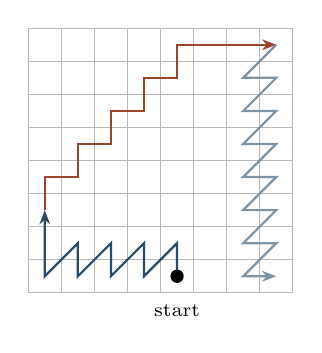
\begin{tikzpicture}[>={Stealth[length=1.8mm]}]
\draw[gray!55, step=0.42] (0,0) grid (3.36,3.36);
\draw[->, thick, inkblue] (1.890,0.210) -- (1.890,0.630) -- (1.470,0.210) -- (1.470,0.210) -- (1.470,0.630) -- (1.050,0.210) -- (1.050,0.210) -- (1.050,0.630) -- (0.630,0.210) -- (0.630,0.210) -- (0.630,0.630) -- (0.210,0.210) -- (0.210,0.630) -- (0.210,1.050);
\draw[->, thick, rust] (0.210,1.050) -- (0.210,1.470) -- (0.630,1.470) -- (0.630,1.890) -- (1.050,1.890) -- (1.050,2.310) -- (1.470,2.310) -- (1.470,2.730) -- (1.890,2.730) -- (1.890,3.150) -- (2.310,3.150) -- (2.730,3.150) -- (3.150,3.150);
\draw[->, thick, inkblue!60] (3.150,3.150) -- (2.730,2.730) -- (3.150,2.730) -- (2.730,2.310) -- (3.150,2.310) -- (2.730,1.890) -- (3.150,1.890) -- (2.730,1.470) -- (3.150,1.470) -- (2.730,1.050) -- (3.150,1.050) -- (2.730,0.630) -- (3.150,0.630) -- (2.730,0.210) -- (3.150,0.210);
\fill[black] (1.890,0.210) circle (2.4pt);
\node[below] at (1.890,-0.02) {\scriptsize start};
\end{tikzpicture}

\caption{Bob's route in Theorem~\ref{thm:bottom} for $n=7$, $a=4$: west along the bottom row,
up the left edge, along the diagonal $x-y=-2$ to the top, then down the right edge. Alice's
choices only decide which side of the diagonal the piece passes on.}
\label{fig:strategy}
\end{figure}

\begin{proof}
\emph{The bottom row.} Bob answers $\D$ to $(a-1,0)$. Suppose the piece is at $(b,0)$ with
$0\le b<a$, after a move of Bob, and the named squares are $(i,0)$ for $b\le i\le a$ and $(i,1)$
for $b<i\le a$. Alice's step $\E$ leads to $(b+1,0)$, which is named, and $\D$ leaves the board,
so she steps $\N$ to $(b,1)$. If $b\ge1$, Bob answers $\D$ to $(b-1,0)$ and the description
holds with $b-1$. If $b=0$, Bob's step $\E$ would lead to $(1,1)$, which is named because
$a\ge1$, so he steps $\N$ to $(0,2)$, which exists because $n\ge2$.

\emph{The diagonal.} Every named square now lies in the two bottom rows, apart from $(0,2)$.
Alice is at $(0,2)$; Bob climbs the line $x-y=-2$ as in Theorem~\ref{thm:diag}. At $(i,i+2)$ with
$i\le n-3$, Alice's $\D$ leads to the previous point of the line (or off the board when $i=0$),
and her steps $\E$, $\N$ lead to $(i+1,i+2)$ and $(i,i+3)$, on the lines $x-y=-1$ and $x-y=-3$
above the bottom two rows, which are unnamed. Bob answers to $(i+1,i+3)$. At $(n-2,n)$ the step
$\N$ leaves the board and $\D$ is named (or off the board when $n=2$), so Alice steps $\E$ to
$(n-1,n)$, and Bob steps $\E$ to the corner $(n,n)$.

\emph{The right-hand edge.} The only named squares in the column $x=n$ are $(n,n)$ and, when
$a=n$, the squares $(n,0)$ and $(n,1)$. Lemma~\ref{lem:sweep} applies with $y=n$: take $m=0$ if
$a<n$, and $m=2$ if $a=n$, when $(n-1,1)$ is named because $1\le n-1\le a$.
\end{proof}

From a bottom-row square Alice's step $\D$ leaves the board, so Theorem~\ref{thm:bottom} gives:

\begin{corollary}\label{cor:bottom}
If $n\ge2$ and a bottom-row square $(a,0)$ with $a\ge1$ is winning, Alice's only winning first
move is $\E$.
\end{corollary}

The bound $n\ge 2$ is needed: on the $2\times 2$ board the square $(1,0)$ is winning through
$\N$, because Bob, back at $(0,1)$, has nowhere to go.

\section{Four squares and the corners}

The same pieces prove the statements of Vepir about these squares.

\begin{theorem}\label{thm:small}
The corners $(n,0)$ and $(0,n)$ are losing for $n\ge2$, the square $(2,0)$ is losing for
$n\ge 2$, and $(2,2)$ is losing for $n\ge 3$.
\end{theorem}

\begin{proof}
From $(n,0)$ Alice's only move is $\N$, so Theorem~\ref{thm:bottom} applies; $(0,n)$ follows by
reflection.

From $(2,0)$ the opening $\N$ loses by Theorem~\ref{thm:bottom}. If $n=2$ the square is a corner.
If $n\ge3$ and Alice opens $\E$ to $(3,0)$, Bob answers $\N$ to $(3,1)$ and climbs the line
$x-y=2$ as in Theorem~\ref{thm:diag}: at each point $(i+2,i)$ with $i\ge1$ the step $\D$ leads to
the previous point, and the steps $\E$, $\N$ lead to unnamed squares beside the line. At
$(n,n-2)$ Alice's only move is $\N$ to $(n,n-1)$, and Bob steps $\N$ to $(n,n)$. No square of the
top row other than $(n,n)$ has been named, so Lemma~\ref{lem:sweep} for the top row finishes.

From $(2,2)$ the openings $\E$ and $\N$ lose by Theorem~\ref{thm:diag}. If Alice opens $\D$ to
$(1,1)$, Bob answers $\D$ to $(0,0)$. Alice steps to $(1,0)$ or $(0,1)$; by reflection take
$(1,0)$. Bob's step $\N$ would reach $(1,1)$, so he steps $\E$ to $(2,0)$. From here the play of
the previous paragraph works unchanged. Alice's two steps from $(2,0)$ both lead to squares from
which Bob reaches $(3,1)$; the climb along $x-y=2$ never meets the named squares $(0,0)$,
$(1,0)$, $(1,1)$, $(2,2)$, which lie on other lines; and the top row is still unused when the
piece reaches $(n,n)$, because $n\ge3$ keeps $(2,2)$ off it.
\end{proof}

\section{Conjectures}

For odd $n$ the boards up to $10\times 10$ follow the pattern that Vepir conjectured, which can
be stated row by row. By the reflection it is enough to describe the squares $(x,y)$ with
$x\ge y$.

\begin{conjecture}\label{conj:even}
Let $n$ be odd. A square $(x,y)$ with $x\ge y$ is losing exactly when
\begin{itemize}
\item $x=y$ and $y$ is even or $y=n$; or
\item $y=1<x$ and $x=n$; or
\item $y$ is even, $y<n$, and $x\ge y+2$; or
\item $y\ge3$ is odd, $x>y$ and $x-y$ is even.
\end{itemize}
\end{conjecture}

Read row by row: on an even row the diagonal square is losing, its east neighbour winning and the
rest of the row losing; on an odd row from $3$ on, losing and winning squares alternate from the
diagonal; row $1$ is winning except at the edge. For $n=1,3,5,7,9$ the conjecture agrees with the
exact solution on every square, and the number of losing squares on the $2m\times 2m$ board it
predicts is $3m^2-4m+5$ for $m\ge 2$. If it holds, Alice wins with probability tending to $1/4$
for odd exponents.

For even $n$ the exceptions in Theorem~\ref{thm:counts} show no pattern yet. Vepir lists
further exceptions on the $11\times 11$ board, which this note has not checked.

\section{What does not work}

Several natural approaches fail, and the reasons are short enough to record.

\emph{Copying.} Bob's move $\E$ after Alice's $\E$, and so on, returns the piece to a square with
both coordinates even after every pair of moves, and on boards with $n$ even it never leaves the
board. It loses on the $3\times3$ board from $(2,0)$: after $\N,\N,\D,\D$ the piece is at
$(0,0)$, Alice steps $\E$ to $(1,0)$, and Bob has no move. Bob wins from $(2,0)$ by answering
the first $\N$ with $\D$ instead.

\emph{Local rules and invariants.} On the boards computed, the right answer for Bob depends on
the shape of the whole unused region. In particular, no rule that weights each square and
compares a total with a threshold, or takes a total modulo $2$, predicts the winner of
positions on the $5\times5$ and $7\times7$ boards; the corresponding linear systems, built from
a few thousand positions labelled by exhaustive search, have no solution. This is consistent
with complexity theory: deciding the winner of the same game on a general directed graph is
PSPACE-complete, even for planar graphs~\cite{LS}.

\emph{Rectangles.} The same game on $R\times C$ boards is regular when $R=3$ and close to the
square pattern when both sides are odd, but boards with an even side, such as $4\times 7$ and
$6\times 9$, show no visible pattern. An induction over rectangles therefore has no statement to
carry, and a proof of Conjecture~\ref{conj:even} probably has to use the reflection symmetry
of the square.

\section*{Data and code}
The solver, an independent second solver, the scripts that check every statement in this note
on boards up to $9\times 9$, and the tables are in the folder of this note at
\url{https://github.com/jvvk/mathematics}. Lemma~\ref{lem:sweep} and Theorems~\ref{thm:diag},
\ref{thm:bottom} and~\ref{thm:small} are also checked, for every board, in the Lean proof assistant.

\section*{Acknowledgements}
The proofs, text and programs were developed with the AI assistant Claude (Anthropic), under the
author's direction. The author thanks Witold and Vepir for the question and their data. The
author is responsible for the contents.

\begin{thebibliography}{9}
\bibitem{LS} D.~Lichtenstein and M.~Sipser, GO is polynomial-space hard, \emph{J. ACM}
\textbf{27} (1980) 393--401, \href{https://doi.org/10.1145/322186.322201}{doi:10.1145/322186.322201}.
\bibitem{MO} Vepir, Players alternate moving a $\{\swarrow,\uparrow,\rightarrow\}$ piece on a
chessboard, MathOverflow question 363120 (2020), \url{https://mathoverflow.net/q/363120},
accessed 10 October 2026.
\bibitem{MSE} Witold, Winning strategy in a game with the positive divisors of $10^n$,
Mathematics Stack Exchange question 3689425 (2020), with an answer by Vepir,
\url{https://math.stackexchange.com/q/3689425}, accessed 10 October 2026.
\bibitem{TYM} XXIII All-Ukrainian Tournament of Young Mathematicians named after M.~Y.~Yadrenko
(2020), problem 20, \url{https://tym.in.ua/}, accessed 10 October 2026.
\end{thebibliography}

\end{document}
